\subsection{Viscosity}
	\begin{figure}[H]
		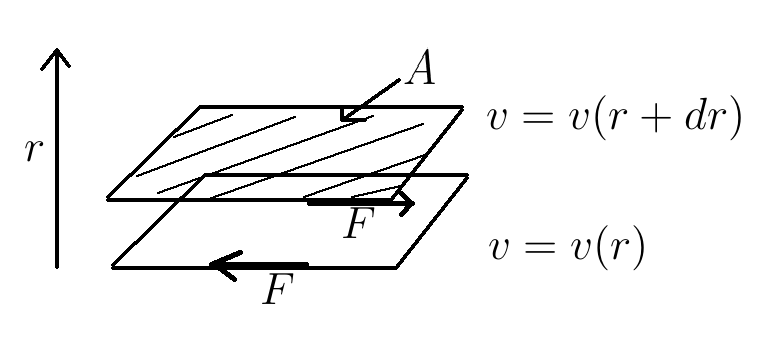
\includegraphics[height=5cm]{fig_diagram-viscosity-def}
		\caption{[NEED CHANGE]Force between two layers of viscous liquid}
		\label{fig_diagram-viscosity-def}
	\end{figure}
	
	Viscosity is defined as,
	
	\begin{equation} \label{eq:def-viscosity}
		\frac{F}{A} = \mu \left| \frac{dv}{dr} \right|
	\end{equation}
	
	\begin{itemize}
		\item $F$: shearing force on a surface of the layer, this force acts parallel to the surface plane.
		\item $A$: the area of the surface.
		\item $\mu$: coefficient of viscosity.
		\item $v$: velocity of the flow parallel to the plane.
		\item $r$: coordinate perpendicular to the plane.
	\end{itemize}
	
	Dimension of viscosity,
	
	\[ [\mu] = \frac{[F]}{[A]} \frac{[r]}{[v]} \]
	
	\[ [\mu] = \frac{[ML/T^2]}{[L^2]} \frac{[L]}{[L/T]} \]
	
	\begin{equation} \label{eq:diamension-mu}
		[\mu] = \frac{M}{LT} = \frac{kg}{m.s}
	\end{equation}


\subsection{Volumetric flow rate through a thin tube}
	
	\begin{figure}[H]
		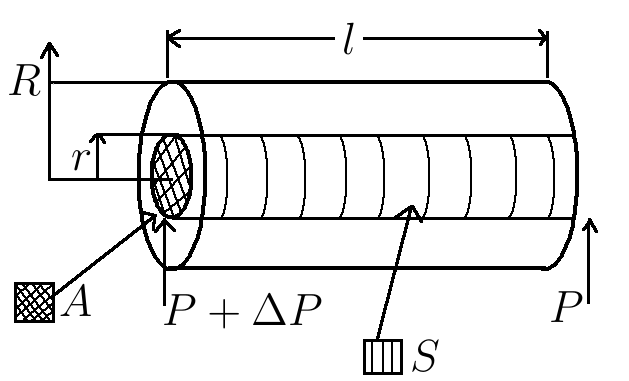
\includegraphics[height=5cm]{fig_flow-thin-tube}
		\caption{[NEED CHANGE]Flow through a thin tube}
		\label{fig_flow-thin-tube}
	\end{figure}
	
	Rearranging \ref{eq:def-viscosity}, the viscous force is given by,
	
	\begin{equation} \label{eq:force-viscous}
		F_{vis} = A \mu \left| \frac{dv}{dr} \right|
	\end{equation}
	
	The force due to pressure gradient, for a cross-sectional area $S$,
	
	\begin{equation} \label{eq:force-pressure-grad}
		F_{p} = S \Delta P
	\end{equation}
	
	For a laminar flow, the force due to pressure gradient is compensated by the viscous resistance in the opposite direction, which also means that the fluid does not acclerate.
	
	\begin{equation} \label{eq:f-p-equals-f-vis}
		F_{p} = F_{vis}
	\end{equation}
	
	Substituting \ref{eq:force-viscous} and \ref{eq:force-pressure-grad} into \ref{eq:f-p-equals-f-vis},
	
	\[ S \Delta P = A \mu \left| \frac{dv}{dr} \right| \]
	
	The velocity is maximum in the centre, and zero at the boundaries. Which implies, that the velocity decreases with increasing radius.
	
	\[ \left| \frac{dv}{dr} \right| = -\frac{dv}{dr} \]
	
	\[ S \Delta P = -A \mu \frac{dv}{dr} \]
	
	Substituting $S = \pi r^2$, and $A = 2 \pi r l$,
	
	\[ (\pi r^2) \Delta P = -(2 \pi r l) \mu \frac{dv}{dr} \]
	
	\[ (r) \Delta P = -(2 l) \mu \frac{dv}{dr} \]
	
	\[ -2dv = \frac{\Delta P}{\mu l} r dr \]
	
	\[ -2 \int dv = \frac{\Delta P}{\mu l} \int r dr \]
	
	\[ -2v + C = \frac{\Delta P}{\mu l} \frac{r^2}{2} \]
	
	At $r = R$, $v = 0$
	\[ -2(0) + C = \frac{\Delta P}{\mu l} \frac{R^2}{2} \]
	
	\[ C = \frac{\Delta P}{\mu l} \frac{R^2}{2} \]
	
	\[ -2v + \left( \frac{\Delta P}{\mu l} \frac{R^2}{2} \right) = \frac{\Delta P}{\mu l} \frac{r^2}{2} \]
	
	\[2v = \frac{\Delta P}{\mu l} \frac{R^2}{2} - \frac{\Delta P}{\mu l} \frac{r^2}{2} \]
	
	\begin{equation} \label{eq:velocity-dist-pou}
		v(r) = \frac{\Delta P}{4 \mu l} (R^2 - r^2)
	\end{equation}
	
	In order to find the volumetric flow rate $Q$ in a tube, we integrate for each thin strip $2 \pi r dr$
	
	\[ Q = \int_{S} vdS = \int_{0}^{R} v(r) (2 \pi r) dr \]
	
	\[ Q = 2 \pi \int_{0}^{R} v(r) r dr \]
	
	Substituting $v(r)$ from \ref{eq:velocity-dist-pou}
	
	\[ Q = 2 \pi \int_{0}^{R} \left( \frac{\Delta P}{4 \mu l} (R^2 - r^2)\right) r dr \]
	
	\[ Q =  \frac{\pi \Delta P}{2 \mu l} \int_{0}^{R} (R^2r - r^3)dr \]
	
	\[ Q =  \frac{\pi \Delta P}{2 \mu l} \left[ \frac{R^2r^2}{2} - \frac{r^4}{4} \right]_{0}^{R} \]
	
	\[ Q =  \frac{\pi \Delta P}{2 \mu l} \left( \frac{R^4}{2} - \frac{R^4}{4} \right) \]
	
	\begin{equation} \label{eq:flow-rate}
		\boxed{Q = \frac{\pi}{8} \frac{\Delta P}{\mu l} R^4}
	\end{equation}

\subsection{Capillary Action}

	\begin{figure}[H]
		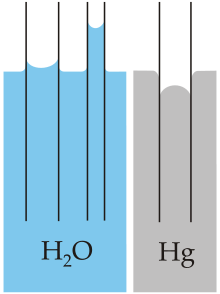
\includegraphics[height=8cm]{fig_capact-of-water}
		\caption{Showing capillary action of water (polar) compared to mercury (non-polar), with respect to a polar surface such as glass (Si–OH).}
		\label{fig_capact-of-water}
	\end{figure}
	
	Let us apply this to our case, where the first node is filled with a fluid like water and the second node is filled with a fluid like air, and the our tube is similar to glass. Hence the meniscus will be oriented in a manner shown below.
	
	\begin{figure}[H]
		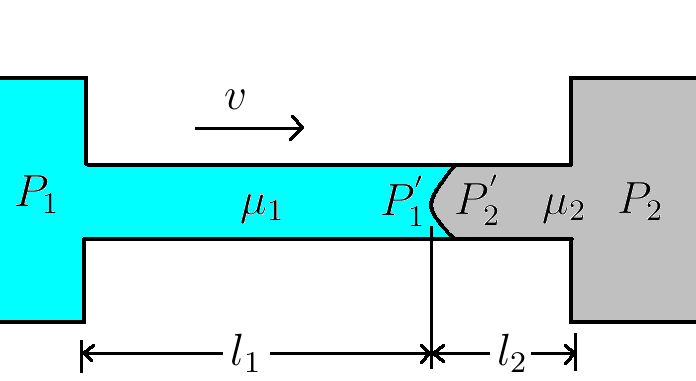
\includegraphics[height=3cm]{fig_shape-meniscus}
		\caption{Orientation of meniscus, when one of its side is filled with wetting fluid while the other side is filled with a non-wetting fluid.}
		\label{fig_shape-meniscus}
	\end{figure}
	
	This causes the water to climb against gravity.
	
	



\subsection{Flow rate in a tube containing 1 meniscus}

	\begin{figure}[H]
		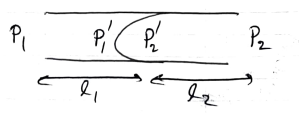
\includegraphics[height=3cm]{fig_flowr-1-men}
		\caption{Pressures in a tube with two phases.}
		\label{fig_flowr-1-men}
	\end{figure}

	Let there be a higher pressure in $P_{1}$ than $P_{2}$, the fluid in node which has $P_{1}$ produces a meniscus which tends to move towards the second node. We can break it down into two separate tubes of lengths $l_{1}$ and $l_{2}$, containing fluid of viscosites ${\mu}_1$ and ${\mu}_2$. Then the flow rates for each of the tubes are given by:
	
	\begin{equation} \label{eq:flow-rate-first}
		Q_1 = \frac{\pi}{8{\mu}_1} \frac{P_1 - P^{'}_1}{l_1} R_1^4
	\end{equation}
	
	\begin{equation} \label{eq:flow-rate-second}
		Q_2 = \frac{\pi}{8{\mu}_2} \frac{P^{'}_2 - P_2}{l_2} R_2^4
	\end{equation}

	Multiplying equations \ref{eq:flow-rate-first} and \ref{eq:flow-rate-second} by ${\mu}_i l_i$
	
	\begin{equation} \label{eq:flow-rate-first-coeff}
		Q_1 {\mu}_1 l_1 = \frac{\pi}{8} (P_1 - P^{'}_1) R_1^4
	\end{equation}
	
	\begin{equation} \label{eq:flow-rate-second-coeff}
		Q_2 {\mu}_2 l_2 = \frac{\pi}{8} (P^{'}_2 - P_2) R_2^4
	\end{equation}

	Due to continuity, which means no vacuum or fluid can be created, $Q_1 = Q_2$. Since it is the same tube, $R_1 = R_2$. Adding equation \ref{eq:flow-rate-first-coeff} and \ref{eq:flow-rate-second-coeff}, we get:
	
	\begin{equation} \label{eq:flow-rate-intermediate}
		Q({\mu}_1 l_1 + {\mu}_2 l_2) = \frac{\pi}{8}R^4(P_1 - P_2 + P^{'}_2 - P^{'}_1)
	\end{equation}

	In figure \ref{fig_capact-of-water} the water rises because there is a pressure jump at the meniscus, the pressure is lower on the side of the water. Therefore in our case $P^{'}_2 - P^{'}_1$ will have a positive value. Equation \ref{eq:flow-rate-intermediate} becomes:
	
	\begin{equation} \label{eq:flow-rate-1mns-basic}
		Q = \frac{\pi R^4}{8({\mu}_1 l_1 + {\mu}_2 l_2)} \left( \Delta P + \frac{2\sigma}{R} \right)
	\end{equation}
	
	It is clear that $Q > Q'$, where $Q'$ is the flow without the meniscius.
	
	
\subsection{The sign of capillary pressure}

	Let the node on which we are generating linear equations be $N_i$ and the node connected by a tube be $N_j$, if the concave side of the meniscus points towards $N_j$ from $N_i$, then let us say that the meniscus points away from $N_i$ or simply points away and in the case of opposite orientation points towards. Let the sign due to the orientation of meniscus be decided by a function called $s(d, n_{mns})$, where $d$ is the direction or orientation, and $n_{mns}$ is the number of meniscus in the tube:
	
	\begin{equation}
		s(d, n_{mns}) = 
		\begin{dcases}
			-1,&\text{points towards, $n_{mns}$ = 1}\\
			0,&\text{$n_{mns}$ = 0, 2}\\
			+1,&\text{points away, $n_{mns}$ = 1}
		\end{dcases}
	\end{equation}

	Equation \ref{eq:flow-rate-1mns-basic} can be written as:
	
	\begin{equation} \label{eq:flow-rate-1mns-complex}
		Q = \frac{\pi R^4}{8({\mu}_1 l_1 + {\mu}_2 l_2)} \left( \Delta P + \frac{2s\sigma}{R} \right)
	\end{equation}
	
	The case when there are an even number of meniscus in a tube, the capillary pressures cancel each other out.

\subsection{Flow rate equation used in our network model}
	\begin{figure}[H]
		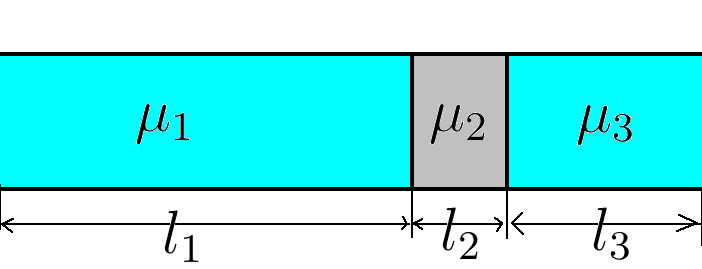
\includegraphics[height=3cm]{fig_tube-length-viscosity-numbering}
		\caption{designation of viscosity and corresponding lengths of phases in a tube}
		\label{fig_tube-length-viscosity-numbering}
	\end{figure}
	
	$Q_{ij}$ is the flow from $N_i$ to $N_j$ and $\Delta P_{ij} = P_i - P_j$.
	
	\begin{equation} \label{eq:flow-rate-main}
		\boxed{Q_{ij} = \frac{\pi R_{ij}^4}{8M_{ij}l} \left(\Delta P_{ij} + \frac{2s_{ij}\sigma}{R_{ij}} \right)}
	\end{equation}
	
	Here $M_{ij}$ is:
	\[ {M}_{ij} = \sum_{k} {\mu}_{ijk} \frac{l_{ijk}}{l} \]
	 
	It is clear that

	\begin{equation}
		Q_{ij} = -Q_{ji}
	\end{equation}


\subsection{Set of linear equations for a node} \label{sec:linear-equ}

	Let us apply our method on a simple system consisting of only 5 nodes. 

	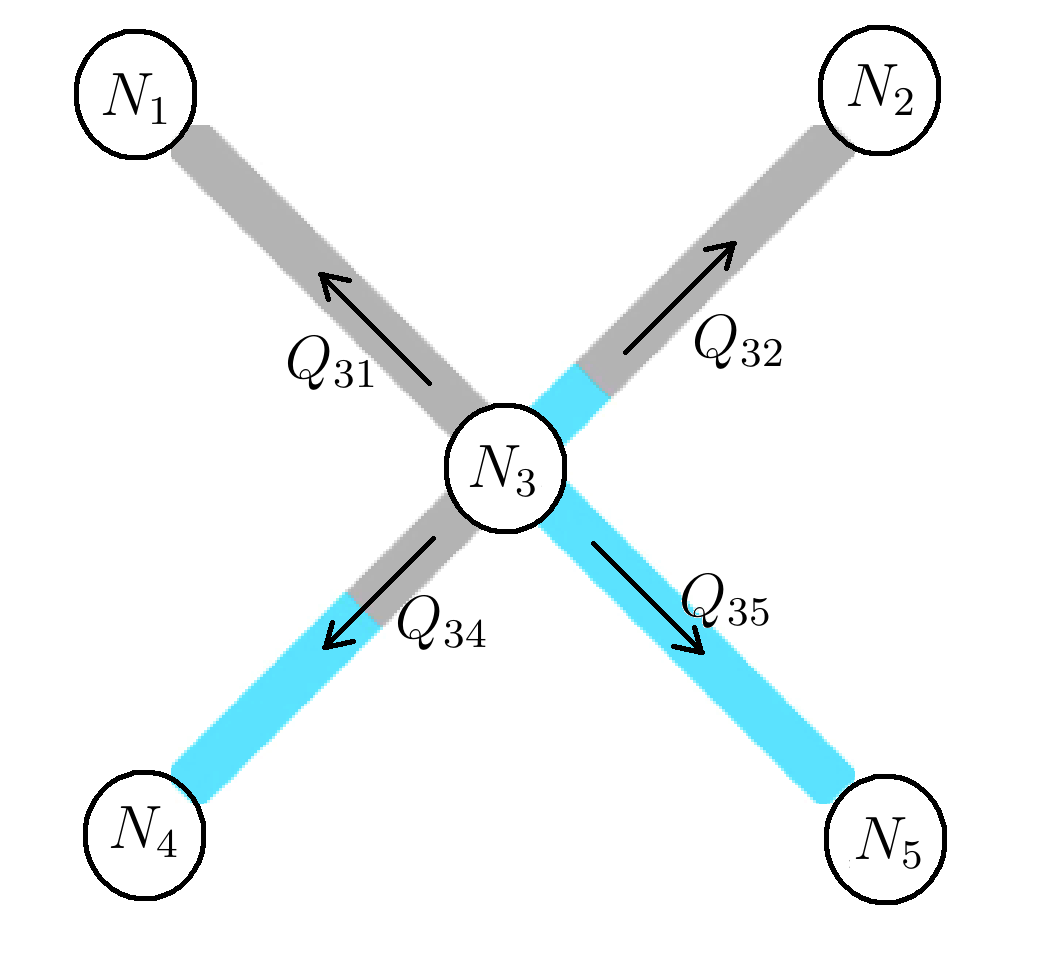
\includegraphics[height=8cm]{figures/fig_simple-5-nodes}

	Since there are 4 tubes, we can write 4 equations according to \ref{eq:flow-rate-main}
	
	\[ Q_{31} = \frac{\pi R_{31}^3}{8lM_{31}}(R_{31}\Delta P_{31} + 2s_{31}\sigma) \]
	\[ Q_{32} = \frac{\pi R_{32}^3}{8lM_{32}}(R_{32}\Delta P_{32} + 2s_{32}\sigma) \]
	\[ Q_{34} = \frac{\pi R_{34}^3}{8lM_{34}}(R_{34}\Delta P_{34} + 2s_{34}\sigma) \]
	\[ Q_{35} = \frac{\pi R_{35}^3}{8lM_{35}}(R_{35}\Delta P_{35} + 2s_{35}\sigma) \]

	Due to the conservation of volume, we have:
	\[ \sum_{k} Q_{3k} = 0 \]
	
	Where $k = {1, 2, 4, 5}$.
	
Here are all the citations \cite{aker1998two}, and \cite{raoof2010new}, \cite{sinha2017effective}, \cite{fatt1956network}	all good.
